% !TeX root = RJwrapper.tex
\title{chemmodlab}
\author{by Jeremy Ash, Jacqueline Hughes-Oliver}

\maketitle

\abstract{%
An abstract of less than 150 words.
}

\section{Introduction}\label{introduction}

{[}TODO this text was written for JCIM and needs to be made less
specific to cheminformatics for r journal{]}

In the recent years, virtual screening technologies have become an
integral part of the discovery pipeline. In this pipeline, fast and
accurate virtual screening methods are necessary to reduce a pool of
compounds on the order of 10 million to a few thousand that are enriched
for potential actives and can be tested experimentally. While only one
approach to virtual screening, QSAR-based methods have become pervasive
in the recent years. Cherkasov et al have recently reviewed {[}REF{]}
numerous recent examples of QSAR-based virtual screening leading to the
experimental identification of novel, highly active compounds. For
example, Zhang et al {[}REF{]} have recently used QSAR models to
virtually screen the ChemBridge library for novel antimalarials. They
confirmed 25 of these predictions experimentally, some of which had
novel scaffolds, opening up new avenues for lead optimization and
further exploration of new antimalarial chemical structures. However
QSAR model performance can vary dramatically and it is often unclear
which modeling method and/or descriptor set will have the best
performance for a particular data set {[}Hopfinger REF{]}. Therefore, it
is often necessary to use multiple modeling routines and compare their
performance with measures of prediction accuracy for held out data.

\begin{itemize}
\tightlist
\item
  Importance of QSAR based virtual screening methods

  \begin{itemize}
  \tightlist
  \item
    Need highly accurate models to screen large databases and locate
    only a few actives
  \item
    Example of how QSAR predictions have been experimentally confirmed
    and identified novel, highly active compounds
  \end{itemize}
\item
  Difficulties with QSAR models

  \begin{itemize}
  \tightlist
  \item
    High dimensional data with many predictors and few observations.
    Non-linear relationships between predictors and response. Models
    must have enough flexibility to adequately capture complex
    relationships.
  \item
    Often unclear which model will have the best performance - need to
    try many
  \item
    However, in Cheminformatics literature only a few modeling
    strategies are typically compared
  \item
    Variability of model accuracy measures with different splits is
    often ignored
  \end{itemize}
\item
  ChemModLab

  \begin{itemize}
  \tightlist
  \item
    State there was previously a webserver and now is an R-package
  \item
    Can now analyze any set of descriptors and can take advantage of
    several nice packages for computing chemical descriptors like RDkit.
  \item
    Goal: Streamline fitting and assessing many QSAR models
  \item
    Implements 12 machine learning models in R (svm, neural nets, random
    forests, etc)
  \item
    Requires little user intervention -- fits all models with one
    command
  \item
    Provides sensible defaults for tuning parameters
  \item
    Users can tune and set parameters manually if they like
  \item
    Fits any subset of these models to any number of descriptor sets the
    user provides
  \item
    Performs repeated k-fold cross-validation to assess model accuracy
  \end{itemize}
\item
  Mention specifically new features that have been implemented

  \begin{itemize}
  \tightlist
  \item
    Implemented many new accuracy measures
  \item
    Users can now customize tuning parameters
  \item
    Parallel processing
  \end{itemize}
\end{itemize}

\section{chemmodlab implementation}\label{chemmodlab-implementation}

\subsection{Overview}\label{overview}

\textbf{chemmodlab} takes advantage of the numerous machine learning
models already implemented in the R environment. Its primary aim is to
streamline the process of model fitting so that users do not have to
learn the syntax and best practices for fitting each model separately.
\textbf{chemmodlab} is organized into two successive components: (1)
model fitting and (2) model assessment.

\subsection{An illustrative example}\label{an-illustrative-example}

We will use a cheminformatics data set to illustrate a typical analysis
pipeline in \textbf{chemmodlab}. In cheminformatics, chemists often
build machine learning models that relate a chemical compound's
structure to an observed endpoint. These models are collectively
referred to as quantitative structure activity relationship (QSAR)
models. See {[}REF{]} for an excellent review of the ways in which these
models have played a crucial role in the drug discovery process. Often
the ``endpoint'' (or response variable) is a measure of a compound's
biological activity, which may be either binary, indicating
active/inactive, or a continuous measure of binding affinity for a
target protein. Chemical ``descriptors'' (also known as predictors,
features, or covariates) represent various levels of organization of a
chemical's structure. See {[}REF{]} for an overview of commonly used
chemical descriptors.

The data we will analyze is from a cytotoxicity assay conducted by the
Scripps Research Institute Molecular Screening Center. There are 3,286
compounds, 50 of which are active. Visit
\url{http://pubchem.ncbi.nlm.nih.gov/assay/assay.cgi?aid=364} for more
details.

For completeness, the preprocessing of the data set analyzed will be
shown. First, the response variable and molecule ID's are read in from
file.

\begin{Schunk}
\begin{Sinput}
data <- read.csv("AID_364_response.csv")
head(data)
\end{Sinput}
\begin{Soutput}
#>        CID Outcome
#> 1  5388992       1
#> 2  5388983       1
#> 3   663143       1
#> 4    10607       1
#> 5  5388972       1
#> 6 11970251       1
\end{Soutput}
\end{Schunk}

Next, two descriptor sets are added to the data frame. Both of these
sets were computed using the software, PowerMV - see {[}REF{]} for more
information. The first set of continuous descriptors are a modification
of the Burden number descriptors {[}REF{]}.

\begin{Schunk}
\begin{Sinput}
desc.lengths <- c()
d <- read.csv("BurdenNumbers.csv")
head(d[, 1:5])
\end{Sinput}
\begin{Soutput}
#>        Row WBN_GC_L_0.25 WBN_GC_H_0.25 WBN_GC_L_0.50 WBN_GC_H_0.50
#> 1  5388992      -2.40010       1.98339      -2.52864       2.50835
#> 2  5388983      -2.40010       1.98240      -2.52868       2.50398
#> 3   663143      -2.41650       1.32890      -2.53910       2.05778
#> 4    10607      -2.38337       2.17677      -2.52643       2.33232
#> 5  5388972      -2.29039       1.97468      -2.41743       2.46177
#> 6 11970251      -2.29039       2.22488      -2.41748       2.56161
\end{Soutput}
\begin{Sinput}
data <- cbind(data, d[-1])
desc.lengths <- c(desc.lengths, ncol(d[-1]))
\end{Sinput}
\end{Schunk}

The number of descriptors in each descriptor set are also stored, as
this information will be used to parse the data frame later on. The
second set contains binary descriptors, indicating the presence/absence
of ``pharmacophore'' features, described in more detail in {[}REF{]}.

\begin{Schunk}
\begin{Sinput}
d <- read.csv("Pharmacophores.csv")
head(d[, 1:6])
\end{Sinput}
\begin{Soutput}
#>        Row NEG_01_NEG NEG_02_NEG NEG_03_NEG NEG_04_NEG NEG_05_NEG
#> 1  5388992          0          0          0          0          0
#> 2  5388983          0          0          0          0          0
#> 3   663143          0          0          0          0          0
#> 4    10607          0          0          0          0          0
#> 5  5388972          0          0          0          0          0
#> 6 11970251          0          0          0          0          0
\end{Soutput}
\begin{Sinput}
data <- cbind(data, d[-1])
desc.lengths <- c(desc.lengths, ncol(d[-1]))

dim(data)
\end{Sinput}
\begin{Soutput}
#> [1] 3311  173
\end{Soutput}
\begin{Sinput}
aid364 <- data
\end{Sinput}
\end{Schunk}

\subsection{\texorpdfstring{Model fitting: The \textbf{ModelTrain}
function}{Model fitting: The ModelTrain function}}\label{model-fitting-the-modeltrain-function}

For the model fitting component of \textbf{chemmodlab}, the primary
function is ModelTrain, which fits a series of classification or
regression models to a data set.

\subsubsection{\texorpdfstring{The \textit{data} input
parameter}{The  input parameter}}\label{the-input-parameter}

This function takes as input a data frame with an (optional) ID column,
a response column, and descriptor columns. We have processed the
\emph{aid364} data set so that it follows this format. The specification
of an ID column allows users to easily match response predictions to
their observation IDs in the \textbf{chemmodlab} output.
\textbf{chemmodlab} can currently handle responses that are continuous
or binary (represented as a numeric vector with 0 or 1 values). Users
can specify which columns in the data frame they would like to consider
distinct descriptor sets. At the moment, the response and descriptors
may only be binary or continuous, though we are currently working on
support for categorical variables of more than two levels.

We previously stored the number of descriptors in each descriptor set in
an integer vector named \textit{desc.lengths}, with the ordering of the
integers matching the order of the descriptor sets in \textit{aid364}:

\begin{Schunk}
\begin{Sinput}
desc.lengths
\end{Sinput}
\begin{Soutput}
#> [1]  24 147
\end{Soutput}
\end{Schunk}

Users can also name the descriptor sets by providing a character vector
to the \textit{des.names} parameter. If this character vector is
specified, all of \textbf{ModelTrain} output and downstream
\textbf{chemmodlab} functions will name the descriptor sets accordingly:

\begin{Schunk}
\begin{Sinput}
des.names = c("BurdenNumbers", "Pharmacophores")
\end{Sinput}
\end{Schunk}

The specification of distinct descriptor sets in a data frame is
illustrated in the following call to \textbf{ModelTrain}:

\begin{Schunk}
\begin{Sinput}
cml <- ModelTrain(aid364, ids = TRUE, xcol.lengths = desc.lengths, 
                  des.names = des.names)
\end{Sinput}
\end{Schunk}

If the descriptor set columns are not identified by the user, ModelTrain
assumes there is one descriptor set, all columns in data except ycol and
the optional ID column.

\subsubsection{chemmodlab models}\label{chemmodlab-models}

Currently, 13 different machine learning models are implemented in
\textbf{chemmodlab}. The details of each modeling method, including
descriptions of the default parameters are provided at
\url{https://jrash.github.io/chemmodlab/} (TODO make this into a table
and put in Supporting Info). Briefly, the current models are: elastic
net, k-nearest neighbors, least angle regression, neural networks,
partial least squares linear discriminant analysis, partial least
squares, principal components regression, ridge regression, random
forest, two implementations of recursive partitioning, and support
vector machines.

Some modeling strategies may not be suitable for both binary and
continous responses. Six of the models have implementations in R that
directly support both binary and continuous responses (both
implementations of recursive partitioning, random forest, k-nearest
neighbors, neural networks, and support vector machines). However, five
methods (least angle regression, ridge regression, elastic net,
principal components regression, and partial least squares) assume that
responses have equal variances and normal distributions. This assumption
is often reasonable for continuous responses, but may be suspect if the
response is binary. However, these models can be viewed as a
modification to linear discriminant analysis and still may be
appropriate for binary responses {[}TODO This point was made in the
former chemmodlab paper, but I am not sure if I follow the arguement{]}.
Binary responses are treated as continuous, resulting in continuous
response predictions that are not restricted to range between 0 and 1. A
threshold can then be applied to obtain a binary predicted response. The
model assessment functions discussed later allow users to select this
threshold. Finally, partial least squares linear discriminant analysis
(PLSLDA) cannot be applied to a continous response, but if the user
wishes to analyze this type of data, a threshold value may be used to
convert a continuous response to a binary one.

In cheminformatics applications, descriptors often show strong
multicollinearity. Since this is often problematic for machine learning
models, we have specifically included several models in
\textbf{chemmodlab} that are known to be resilient to multicollinearity
(eg. principal components regression and partial least squares
regression). However, some methods for which prediction is not
considerably affected by multicollinearity do suffer in terms of model
interpretability (eg. recursive partitioning and random forests).

\textbf{chemmodlab} has been designed in a way that it is easily
extensible to new machine learning modeling methods, and new modeling
methods will be added as the authors identify those that have broad
utility to our users. Support for other models can be requested here:
\url{https://github.ncsu.edu/jrash/chemmodlab/issues}.

\textbf{chemmodlab} automatically performs data preprocessing before
fitting the models that require it (eg. centering and scaling variables
before principal components regression), so the user need not worry
about preprocessing of descriptors prior to model fitting.

\subsubsection{\texorpdfstring{Specifying model parameters with
\textit{user.params}}{Specifying model parameters with }}\label{specifying-model-parameters-with}

Sensible default values are selected for each tunable model parameter,
however users may set any parameter manually using the
\textit{user.params} parameter.

\textit{MakeModelDefaults} is a convenience function that makes a list
containing the default parameters fDor all models implemented in
ModelTrain. Users may set any parameter manually by generating a list
with this function and modifying the parameters assigned to each
modeling method:

\begin{Schunk}
\begin{Sinput}
params <- MakeModelDefaults(n = nrow(aid364),
 p = ncol(aid364[, -c(1, 2)]), classify = TRUE, nfolds = 10)
params[1:3]
\end{Sinput}
\begin{Soutput}
#> $NNet
#>   size decay
#> 1    2     0
#> 
#> $PCR
#> NULL
#> 
#> $ENet
#>   lambda
#> 1      1
\end{Soutput}
\begin{Sinput}
params$NNet$size <- 10
params[1:3]
\end{Sinput}
\begin{Soutput}
#> $NNet
#>   size decay
#> 1   10     0
#> 
#> $PCR
#> NULL
#> 
#> $ENet
#>   lambda
#> 1      1
\end{Soutput}
\end{Schunk}

This list can then be provided to the \textit{user.params} parameter to
assign the tuning parameter values used by \textbf{ModelTrain}:

\begin{Schunk}
\begin{Sinput}
cml <- ModelTrain(USArrests, models = "NNet", nsplits = 3,
 user.params = params)
\end{Sinput}
\end{Schunk}

\subsection{Model assessment}\label{model-assessment}

\subsubsection{Repeated k-fold
cross-validation}\label{repeated-k-fold-cross-validation}

For each descriptor set, \textbf{ModelTrain} performs repeated k-fold
cross validation for the selected set of regression and/or
classification models.

For each cross-validation split, observations are randomly assigned to
one of \(k\) folds, splitting the data set into \(k\) blocks that are
approximately equal in size. The number of cross validation folds
(\(k\)) is set with the \textit{nfolds} parameter. Users may also use
the \textit{seed.in} parameter to set the seed for each split, so that
the \textbf{ModelTrain} results are reproducible. Each block is
iteratively held out as a test set, while the remaining \(k-1\) blocks
are used to train each descriptor set and modeling method (D-M)
combination. Predictions for the held out test set are then made with
the resulting models.

Many resampling methods for assessing model performance involve
partitioning a data set into a training set and test set. With these
methods, predictions are made on observations that are not involved in
training. This results in model performance measures that are less
likely to reward over-fitting.

Since performance measures can be highly variable \citep{James2013}
depending on which observations are held out and which are involved in
training, the repetition of this procedure during k-fold cross
validation and the averaging of the performance measures often result in
a more accurate estimation of model performance than a one-time split.

Finding the right number of cross-validation folds for the estimation of
a performance measure involves consideration of the
\textbf{bias-variance trade off}. The mean squared error of an
estimator, a measure of how accurately an estimator estimates the true
value of parameter, can be partitioned into two components, bias and
variance:

\[E[\hat{\theta} - \theta] = (E[\hat{\theta}] - \theta)^2 + Var[\theta]\]

Where \(\hat{\theta}\) is the estimate of the true performance measure
\(\theta\). The first component is bias and the second is variance. An
increase in either the bias or variance will decrease the quality of an
estimator. When a resampling method substantially over- or
under-estimates a performance measure on average, it is said to have
high \textbf{bias}. Bias is often related to size of the data set that
is held out as a test set \citep{James2013}. The smaller the number of
folds in k-fold cross validation, the more observations are held out in
each fold, and the less observations that are used to train a model.
Fewer observations in a training set means that a model is likely to
perform worse, and model performance tends to be underestimated. Thus,
performing k-fold cross validation with 2 folds, where there is 50\% of
the data in each fold, would likely result in high bias.

In contrast, a performance measure estimator suffers from high
\textbf{variance} when its estimate varies considerably when there are
slight changes made to the training and/or test set.
Leave-One-Out-Cross-Validation (LOOV) refers to k-fold cross validation
with \(k\) equal to \(n\), the number of observations. LOOCV often
suffers from high variance \citep{James2013}. This is due to the fact
that the training set changes very little with each iteration of LOOCV.
Thus, performance measure estimates tend be highly correlated. The mean
of a highly correlated variable has higher variance than an uncorrelated
one. Decreasing the number of folds tends to decrease the correlation of
performance measure estimates and lower the variance. Therefore, the
ideal number of folds to use for cross validation is often somewhere
between 2 and \(n\). The number of folds often used for k-fold cross
validation are 5 and 10, as these values frequently provide a good
balance between bias and variance.

Several studies \citep{Molinaro2005, Kim2009, Shen2011} have shown that
repeated cross validation can reduce the variance for a k-fold cross
validation procedure with low bias, achieving a more accurate estimation
of model performance. When k-fold cross validation is repeated in
\textbf{chemmodlab}, multiple iterations of random fold assignment, or
``splits'', are performed. Because the observed performance measures may
vary greatly depending on the definition of folds during k-fold cross
validation, all models are built using the same fold assignment, thus
using fold definition as a ``blocking factor'' in the assesment
investigation. This process is repeated for multiple k-fold cross
validation runs. The user may choose the number of these splits with the
\textit{nsplit} parameter.

We will see later how, in addition to increased accuracy in estimation
of performance measures, repeated cross validation allows one to measure
the standard error of model performance measures, quantifying how
sensitive performance measures are to fold assignments.

\subsubsection{Accumulation curves}\label{accumulation-curves}

\textbf{plot.chemmodlab} takes a \textbf{chemmodlab} object output by
the \textbf{ModelTrain} function and creates a series of accumulation
curve plots for assessing model performance.

The accumulation curve for binary responses shows the number of
positives versus the number of ``tests'' performed, where testing order
is determined by the k-fold cross validated predicted probability of a
response being positive.

The \emph{max.select} parameter sets the maximum number of tests to plot
for the accumulation curves. By default,
\(\left \lfloor{{\min(300, \frac{n}{4})}}\right \rfloor\) is used, where
n is the number of observations. This prioritizes finding actives in a
relatively small number of tests.

Two series of plots are constructed. In the first series, there is one
plot per CV split and descriptor set combination. The accumulation
curves for each model are plotted together so that they can be compared.
In the second plot series, there is one plot per CV split and model fit.
The accumulation curves for each descriptor set are plotted together so
that they can be compared.

By default a large number of accumulation curve plots are constructed.
The \emph{splits} and \emph{meths} parameters may be used to select a
subset of splits and/or methods to plot.

\begin{Schunk}
\begin{Sinput}
plot(cml, splits = 1, meths = c("NNet"))
\end{Sinput}

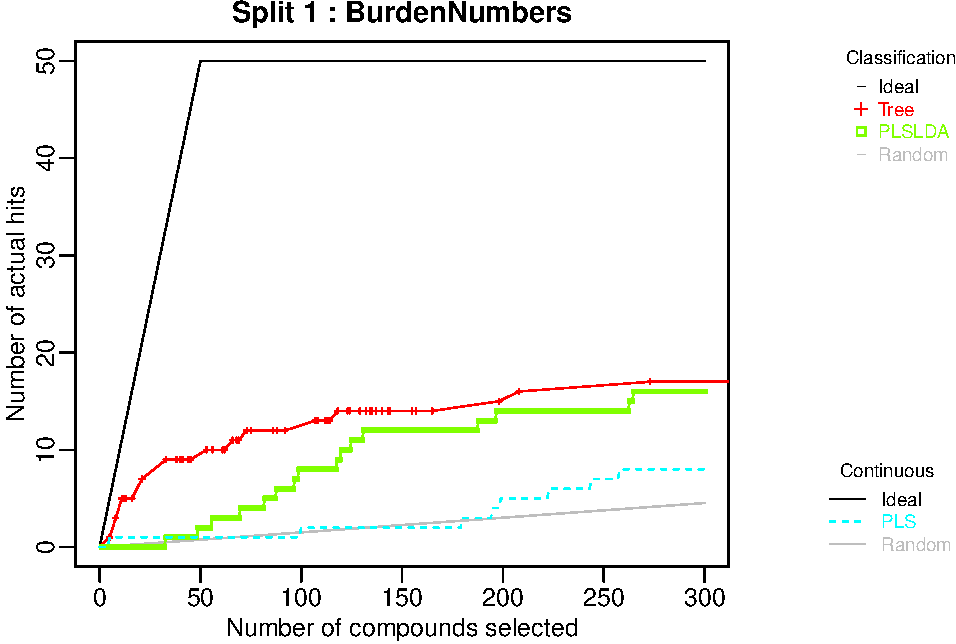
\includegraphics{chemmodlabRJournal_files/figure-latex/accumulation_curves-1} 
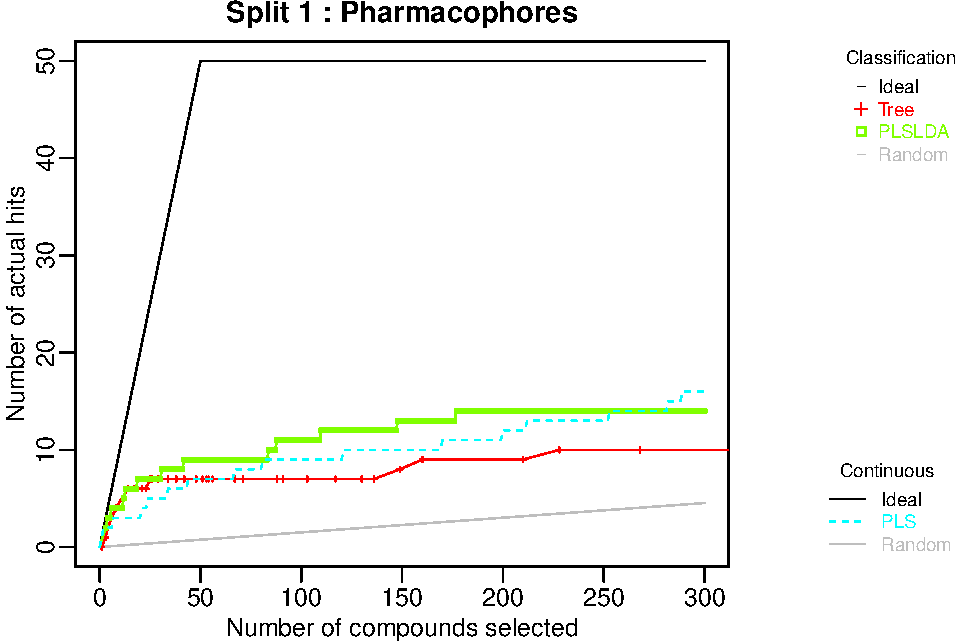
\includegraphics{chemmodlabRJournal_files/figure-latex/accumulation_curves-2} \end{Schunk}

An ``ideal'' curve is plotted on these graphs to demonstrate the
accumulation curve of a model that correctly identifies the \(p\)
positives in the first \(p\) tests. Thus, at \(n\) tests, models with
accumulation curves that are nearest to the ideal curve are preferable.
Also, if an accumulation curve has a slope that is parallel to the ideal
curve for an interval of tests, the model has ideal performance for that
interval. A ``random'' curve shows the accumulation curve if the testing
order were decided at random. At \(n\) tests, models with accumulation
curves that are below the random curve have worse performance than
random chance.

The accumulation curve has also been extended to continuous responses.
In QSAR models, a continuous response is often a measure of binding
affinity (eg. pKi) where a large positive value is preferable.
Therefore, observations on the x-axis are in decreasing order according
to the response. The response is then accumulated so that
\(\sum_{i=1}^{m} y_i\) is the sum of the \(y\) over the first \(m\)
tests. The binary response accumulation curve is a special case of this.

\subsubsection{Multiple comparisons
plots}\label{multiple-comparisons-plots}

Observed performance measures are assessed across all splits using
\textbf{CombineSplits}. This function assesses how sensitive performance
measures are to fold assignments, or small changes to the training and
test sets. Multiplicity-adjusted statistical tests are used to determine
the best performing D-M combination. Intuitively, this assesses how much
a performance measure may change if a slightly different data set is
used.

As input, \textbf{CombineSplits} takes a \textbf{chemmodlab} object
produced by the \textbf{ModelTrain} function:

\begin{Schunk}
\begin{Sinput}
CombineSplits(cml)
\end{Sinput}
\begin{Soutput}
#>    Analysis of Variance on: 'enhancement'
#>  Using factors: Split and Descriptor/Method combination
#> Source    DF         SS         MS          F   p-value   
#> Model      7   11.71832    1.67405   19.19644    <.0001   
#> Error     10    0.87206    0.08721   
#> Total     17   12.59038   
#>       R-Square   Coef Var   Root MSE       Mean   
#>         0.9307     9.3424     0.2953     3.1609   
#> Source       DF       SS       MS        F   p-value   
#> Split         2    0.598    0.299    3.431    0.0486   
#> Desc/Meth     5   11.120    2.224   25.502    <.0001
\end{Soutput}

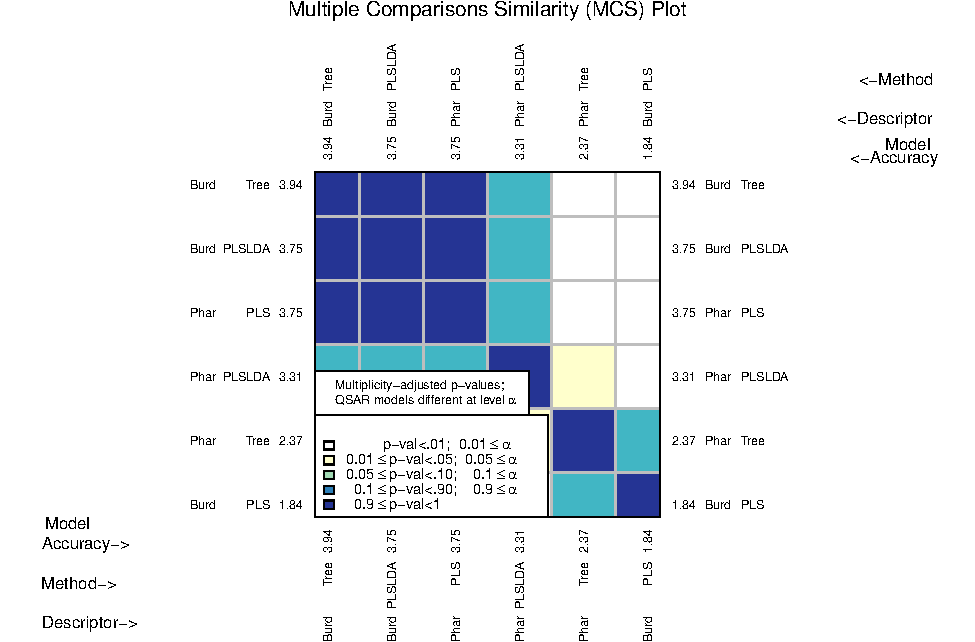
\includegraphics{chemmodlabRJournal_files/figure-latex/CombineSplits_ie-1} \end{Schunk}

By default, \textbf{CombineSplits} uses initial enhancement proposed by
Kearsley et al. {[}REF{]} to assess model performance. Initial
enhancement at \(n\) tests is the hit rate - the fraction of accumulated
positives at \(n\) tests - divided by the porportion of positives in the
entire data set. This is a measure hit rate improvement for a model
relative to random chance. A desirable model will have an initial
enhancement much larger than one. A typical number of tests for initial
enhancement is \(n=300\).

\textbf{CombineSplits} is a designed experiment with two factors: method
(D-M combination) and split (fold assignment). Therefore, we perform an
analysis of variance (ANOVA) to identify significant differences between
the mean performance measures according to factor levels. The linear
model corresponding to this ANOVA is:

\[Y_{ijk} = \mu + \alpha_i + \beta_j + \epsilon_{ijk}\]

Where \(\alpha_i\) corresponds to ith level of the split factor
\(\alpha\) and \(\beta_j\) to the jth level of the method factor
\(\beta\). From the ANOVA table in this example, the split factor is
highly significant, indicating that there is a significant difference
between mean split performance measures for a fixed method. The
difference between mean method performance measures is also highly
significant for a fixed split. The ``error MS'' estimates the variance
in the performance measures within the groups corresponding to each
combination of factor levels. The ``treatment MS'' estimates the
variance between groups.

{[}TODO From the ChemModLab paper: `ChemModLab is a designed study in
that we defined ``experimental'' conditions according to two factors:
modeling method (allowed to take 12 ``levels'') and descriptor set
(allowed to take five ``levels'')\ldots{}.To broaden our range of
inference, we include assay as a third factor. Recognizing that the
definition of folds in k-fold cross validation may have an impact on
observed IE, fold definition is treated as a blocking factor.'

From looking at the code, I believe that there should be two factors,
split and D-M combination. Has the definition of the factors changed
from the way they were defined in the ChemModLab paper? Also With this
data set, we are fitting 16 models, with 2 descriptor sets and 3 splits.
So, shouldnt there be 32-1 = 31 df for the D-M combination factor, and
3-1 = 2 df for the split factor? From the ANOVA tables it seems that the
two factors are split and method. It seems that the degrees of freedom
match this definition of factors (15 for the method factor and 2 for the
split factor). Is there a potentially a bug in the code?{]}

The multiple comparisons plot shows the results for tests for
significance in all pairwise differences of mean model performance
measures. Because there can be many estimated mean performance measures,
an adjustment for multiple testing is necessary. We use the Tukey-Kramer
multiple comparison procedure (see Tukey {[}REF{]} and Kramer
{[}REF{]}). If you are having trouble viewing all the components of the
plot, make the plotting window larger.

For many applications, user may know the number of tests they would like
to perform. This is often the case in drug discovery when chemists have
a set number of compounds they would like to assay and the goal is to
enrich this set of compounds with as many actives as possible. The
number of tests used for initial enhancement may be modified with the
\emph{at} parameter:

\begin{Schunk}
\begin{Sinput}
CombineSplits(cml, at = 100)
\end{Sinput}
\begin{Soutput}
#>    Analysis of Variance on: 'enhancement'
#>  Using factors: Split and Descriptor/Method combination
#> Source    DF        SS        MS         F   p-value   
#> Model      7   87.9341   12.5620   38.8511    <.0001   
#> Error     10    3.2334    0.3233   
#> Total     17   91.1674   
#>       R-Square   Coef Var   Root MSE       Mean   
#>         0.9645    10.5718     0.5686     5.3787   
#> Source       DF       SS       MS        F   p-value   
#> Split         2    4.231    2.116    6.543    0.0111   
#> Desc/Meth     5   83.703   16.741   51.774    <.0001
\end{Soutput}

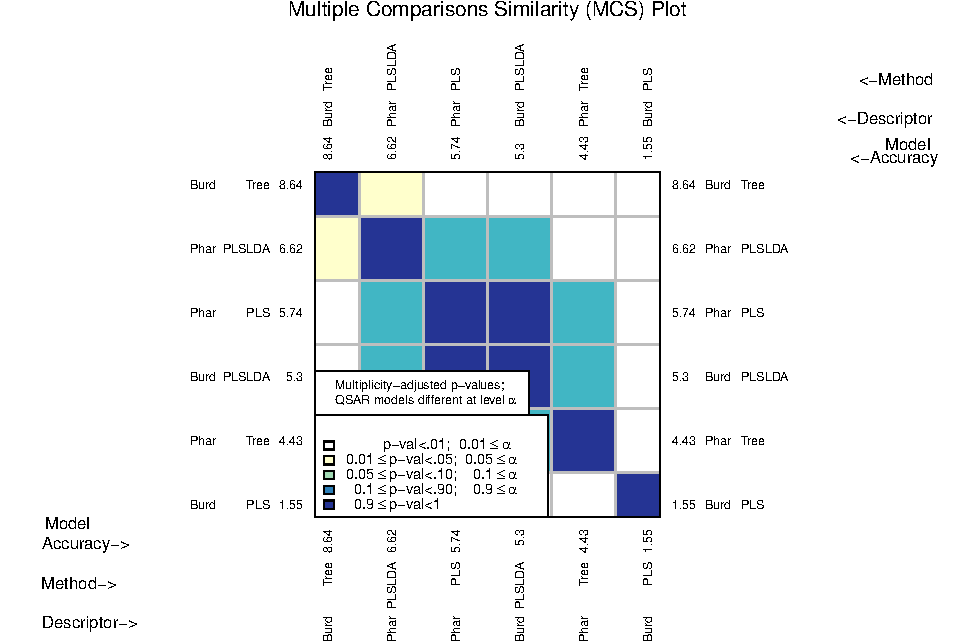
\includegraphics{chemmodlabRJournal_files/figure-latex/CombineSplits_ie_100-1} \end{Schunk}

For binary responses, model performance may also be assessed with
misclassification rate:

\begin{Schunk}
\begin{Sinput}
CombineSplits(cml, metric = "error rate")
\end{Sinput}
\begin{Soutput}
#>    Analysis of Variance on: 'error rate'
#>  Using factors: Split and Descriptor/Method combination
#> Source    DF          SS          MS           F   p-value   
#> Model      7   1.132e-04   1.617e-05   3.702e+01    <.0001   
#> Error     10   4.368e-06   4.368e-07   
#> Total     17   1.176e-04   
#>       R-Square   Coef Var   Root MSE       Mean   
#>       0.962846   3.903900   0.000661   0.016930   
#> Source       DF         SS         MS          F   p-value   
#> Split         2   8.01e-07   4.00e-07   9.16e-01    0.3352   
#> Desc/Meth     5   1.12e-04   2.25e-05   5.15e+01    <.0001
\end{Soutput}

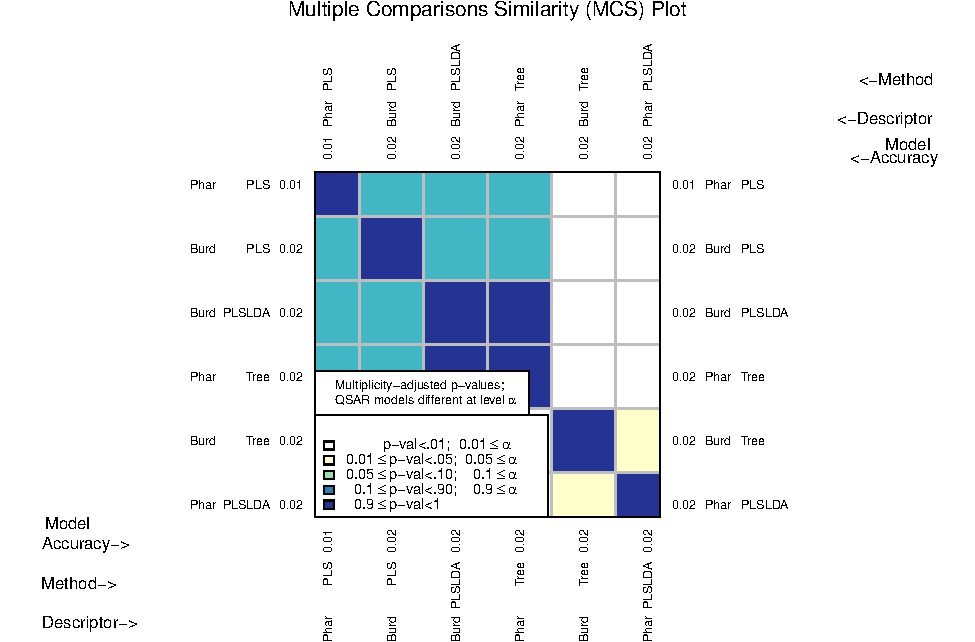
\includegraphics{chemmodlabRJournal_files/figure-latex/CombineSplits_er-1} \end{Schunk}

However, this measure may be inappropriate because it equally penalizes
to false positives and false negatives. In this particular example,
error rate does not do a good job at distinguishing the best performing
models, as the set of plausibly best performing models (the group of
models that do not show a significant performance measure difference
from the best performing model) is quite large:

\begin{Schunk}
\begin{Sinput}
CombineSplits(cml, metric = "specificity")
\end{Sinput}
\begin{Soutput}
#>    Analysis of Variance on: 'specificity'
#>  Using factors: Split and Descriptor/Method combination
#> Source    DF          SS          MS           F   p-value   
#> Model      7   2.210e-04   3.157e-05   3.346e+01    <.0001   
#> Error     10   9.435e-06   9.435e-07   
#> Total     17   2.304e-04   
#>       R-Square   Coef Var   Root MSE       Mean   
#>       0.959048   0.097413   0.000971   0.997138   
#> Source       DF         SS         MS          F   p-value   
#> Split         2   2.54e-06   1.27e-06   1.35e+00    0.2215   
#> Desc/Meth     5   2.18e-04   4.37e-05   4.63e+01    <.0001
\end{Soutput}

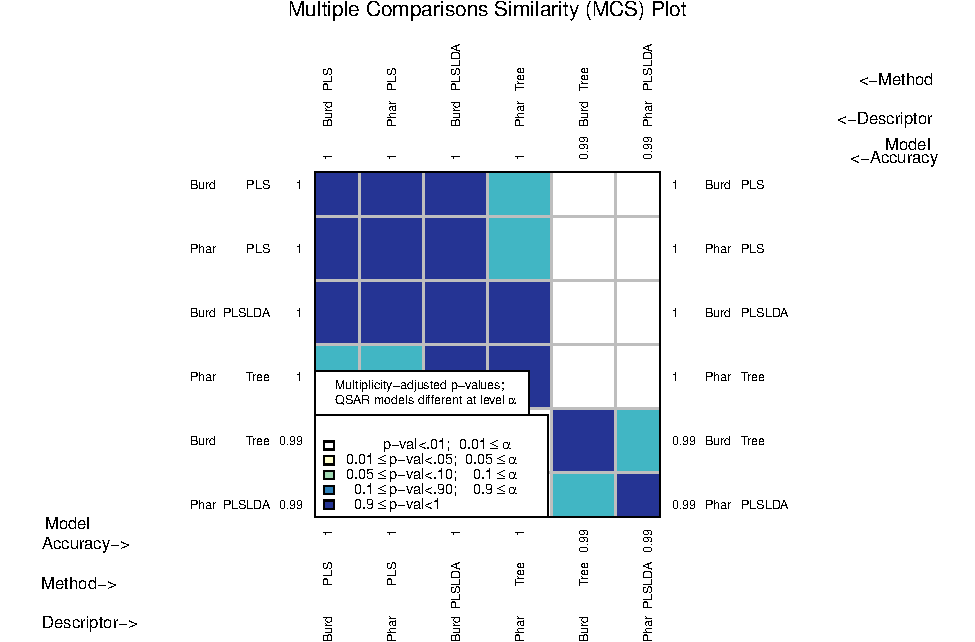
\includegraphics{chemmodlabRJournal_files/figure-latex/CombineSplits_sp-1} \end{Schunk}

This is due to the fact that there are many models that have an average
specificity that is similar to the best performing model. Sensitivity,
however, distinguishes the best performing model much better:

\begin{Schunk}
\begin{Sinput}
CombineSplits(cml, metric = "sensitivity")
\end{Sinput}
\begin{Soutput}
#>    Analysis of Variance on: 'sensitivity'
#>  Using factors: Split and Descriptor/Method combination
#> Source    DF          SS          MS           F   p-value   
#> Model      7   8.189e-02   1.170e-02   2.686e+01    <.0001   
#> Error     10   4.356e-03   4.356e-04   
#> Total     17   8.624e-02   
#>       R-Square   Coef Var   Root MSE       Mean   
#>         0.9495    31.8355     0.0209     0.0656   
#> Source       DF         SS         MS          F   p-value   
#> Split         2    0.00231    0.00116    2.65306    0.0795   
#> Desc/Meth     5    0.07958    0.01592   36.54082    <.0001
\end{Soutput}

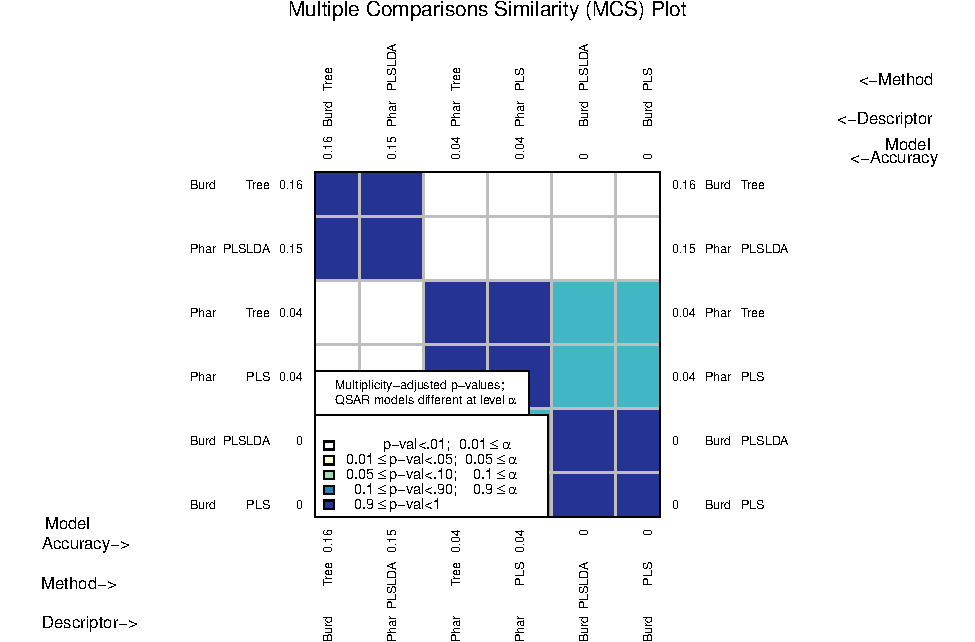
\includegraphics{chemmodlabRJournal_files/figure-latex/CombineSplits_se-1} \end{Schunk}

This example illustrates how using misclassification rate can be
misleading if this is the only model performance measure.
Missclassification rate suggests several models have the best
performance, but these models actually have low sensitivity. In fact,
all of these models identify only a small fraction of the 50 true
positives in the dataset. In the context of drug discovery, sensitivity
measures the percentage of compounds that were correctly predicted to be
active. If the goal of experimental chemists is to correctly identify as
many active compounds as possible, models with low sensitivity may be
less than ideal. The SVM model with Burden number descriptors clearly is
the only model with the highest sensitivity, and may best perform the
task at hand (despite its higher missclassification rate).

The area under the receiver operating characteristic curve (ROC) has
also been implemented in \textbf{chemmodlab}:

\begin{Schunk}
\begin{Sinput}
CombineSplits(cml, metric = "auc")
\end{Sinput}
\begin{Soutput}
#>    Analysis of Variance on: 'auc'
#>  Using factors: Split and Descriptor/Method combination
#> Source    DF          SS          MS           F   p-value   
#> Model      7   0.0167784   0.0023969   6.4754420    0.0026   
#> Error     10   0.0037016   0.0003702   
#> Total     17   0.0204800   
#>       R-Square   Coef Var   Root MSE       Mean   
#>         0.8193     2.8329     0.0192     0.6791   
#> Source       DF        SS        MS         F   p-value   
#> Split         2   0.00307   0.00153   4.14205    0.0327   
#> Desc/Meth     5   0.01371   0.00274   7.40880    0.0019
\end{Soutput}

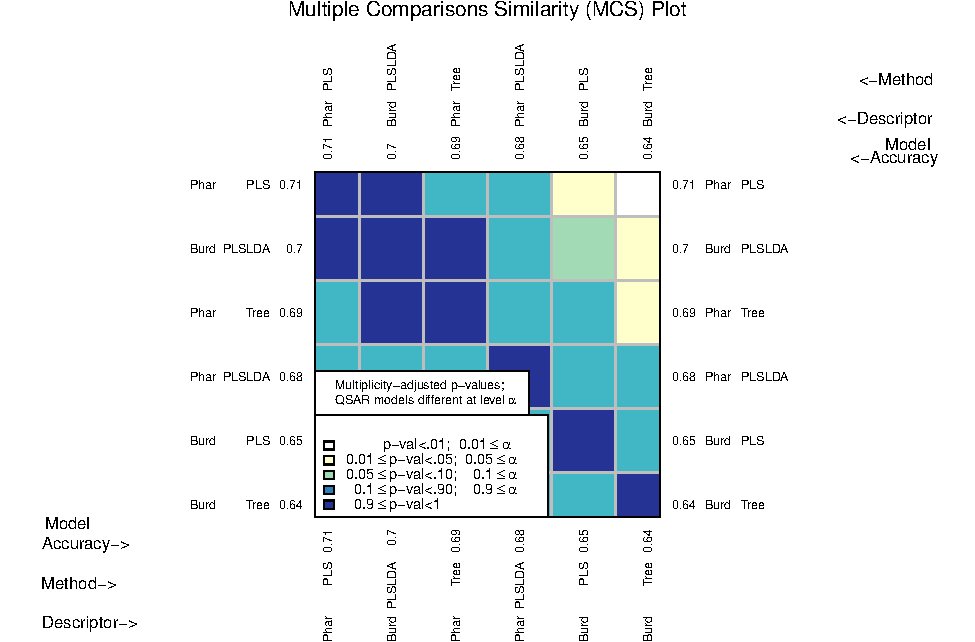
\includegraphics{chemmodlabRJournal_files/figure-latex/CombineSplits_auc-1} \end{Schunk}

Several performance measures have been included for continuous
responses. Though root mean squared error (RMSE) is used broadly in
statistics, it may not be suitable for continuous chemical assay
responses used in cheminformatics. This is because under-predicting and
over-predicting biological activity is equally penalized. An appropriate
alternative may be initial enhancement. Other options are the
coefficient of determination (\(R^2\)) and Spearman's \(\rho\).

\section{Results}\label{results}

\subsection{Summary}\label{summary}

This file is only a basic article template. For full details of
\emph{The R Journal} style and information on how to prepare your
article for submission, see the
\href{https://journal.r-project.org/share/author-guide.pdf}{Instructions
for Authors}. \bibliography{biblio}

\address{%
Jeremy Ash\\
Department of Bioinformatics, Department of Statistics, North Carolina
State University\\
Raleigh, NC 27695-8203, USA\\
}
\href{mailto:jrash@ncsu.edu}{\nolinkurl{jrash@ncsu.edu}}

\address{%
Jacqueline Hughes-Oliver\\
Department of Statistics, North Carolina State University\\
Raleigh, NC 27695-8203, USA\\
}
\href{mailto:hughesol@ncsu.edu}{\nolinkurl{hughesol@ncsu.edu}}

